% PhotonWeave lab-meeting slides, 20-minute version.
% The full deck is photonweave-lab-meeting.tex; both share preamble.tex and figures/.
% Compile with XeLaTeX (Korean text): xelatex photonweave-lab-meeting-20min.tex
\documentclass[aspectratio=169,11pt]{beamer}

% Shared preamble for the PhotonWeave lab-meeting decks.
% Used by photonweave-lab-meeting.tex (full) and
% photonweave-lab-meeting-20min.tex (short). Compile with XeLaTeX.

\usetheme{metropolis}
\metroset{numbering=fraction, progressbar=frametitle, block=fill, sectionpage=progressbar}

\usepackage{fontspec}
\usepackage{kotex}
\usepackage{graphicx}
\usepackage{booktabs}
\usepackage{array}
\usepackage{amsmath}
\usepackage{tikz}
\usepackage{listings}
\usetikzlibrary{arrows.meta, positioning, calc, fit, backgrounds, shapes.geometric,
                decorations.pathreplacing, patterns, shadows.blur}

% ---------------------------------------------------------------- fonts ----
% Korean text falls back gracefully when a font is missing on another machine.
\IfFontExistsTF{NanumBarunGothic}{%
  \setmainhangulfont{NanumBarunGothic}\setsanshangulfont{NanumBarunGothic}}{%
  \IfFontExistsTF{NanumGothic}{\setmainhangulfont{NanumGothic}\setsanshangulfont{NanumGothic}}{}}
\IfFontExistsTF{NanumGothicCoding}{\setmonohangulfont{NanumGothicCoding}}{}

% --------------------------------------------------------------- colours ---
\definecolor{pwdeep}{HTML}{123F66}
\definecolor{pwblue}{HTML}{1F6FB2}
\definecolor{pwsky}{HTML}{6FA8D0}
\definecolor{pwred}{HTML}{D0553F}
\definecolor{pwgreen}{HTML}{3F8F63}
\definecolor{pwamber}{HTML}{E0A300}
\definecolor{pwgrey}{HTML}{8BA0B3}
\definecolor{pwpaper}{HTML}{F3F6F9}

\setbeamercolor{frametitle}{bg=pwdeep, fg=white}
\setbeamercolor{progress bar}{fg=pwblue, bg=pwsky!40}
\setbeamercolor{alerted text}{fg=pwred}
\setbeamercolor{block title}{bg=pwpaper, fg=pwdeep}
\setbeamercolor{block body}{bg=pwpaper!60, fg=black}
\setbeamercolor{title separator}{fg=pwblue}

\newcommand{\hl}[1]{\textcolor{pwdeep}{\textbf{#1}}}
\newcommand{\num}[1]{\textcolor{pwblue}{\textbf{#1}}}
\newcommand{\caveat}[1]{{\footnotesize\textcolor{pwgrey}{#1}}}
\newcommand{\source}[1]{\vspace{2pt}{\scriptsize\textcolor{pwgrey}{출처: #1}}}

% ------------------------------------------------------------- listings ----
\lstset{
  basicstyle=\ttfamily\scriptsize,
  keywordstyle=\color{pwdeep}\bfseries,
  commentstyle=\color{pwgrey}\itshape,
  stringstyle=\color{pwgreen},
  showstringspaces=false,
  columns=fullflexible,
  breaklines=true,
  language=Python,
  frame=none,
  aboveskip=4pt, belowskip=2pt,
}

% -------------------------------------------------------------- helpers ----
% A compact "metric card" used on summary slides.
\newcommand{\card}[3]{%
  \begin{tikzpicture}
    \node[draw=pwsky!60, fill=pwpaper, rounded corners=3pt, inner sep=6pt,
          text width=#1, align=center] {%
      {\color{pwdeep}\bfseries\large #2}\\[2pt]{\scriptsize #3}};
  \end{tikzpicture}}

\metroset{sectionpage=none}

\title{PhotonWeave}
\subtitle{Lumerical FDTD를 대체하는 GPU 가속 FDTD 워크벤치}
\author{Hyoseok Park}
\date{랩미팅 · 2026년 9월}

\begin{document}

% --------------------------------------------------------------- 1. title --
{\setbeamertemplate{footline}{}
\begin{frame}[plain]
  \vspace{-2mm}
  \begin{center}
    {\Huge\bfseries\color{pwdeep} PhotonWeave}\\[4pt]
    {\large Lumerical FDTD를 대체하는 GPU 가속 FDTD 워크벤치}\\[8pt]
    {\footnotesize 브라우저 CAD + Python API + NVIDIA CUDA 네이티브 솔버\quad·\quad MIT 라이선스\quad·\quad v0.14.0.dev}\\[8pt]
    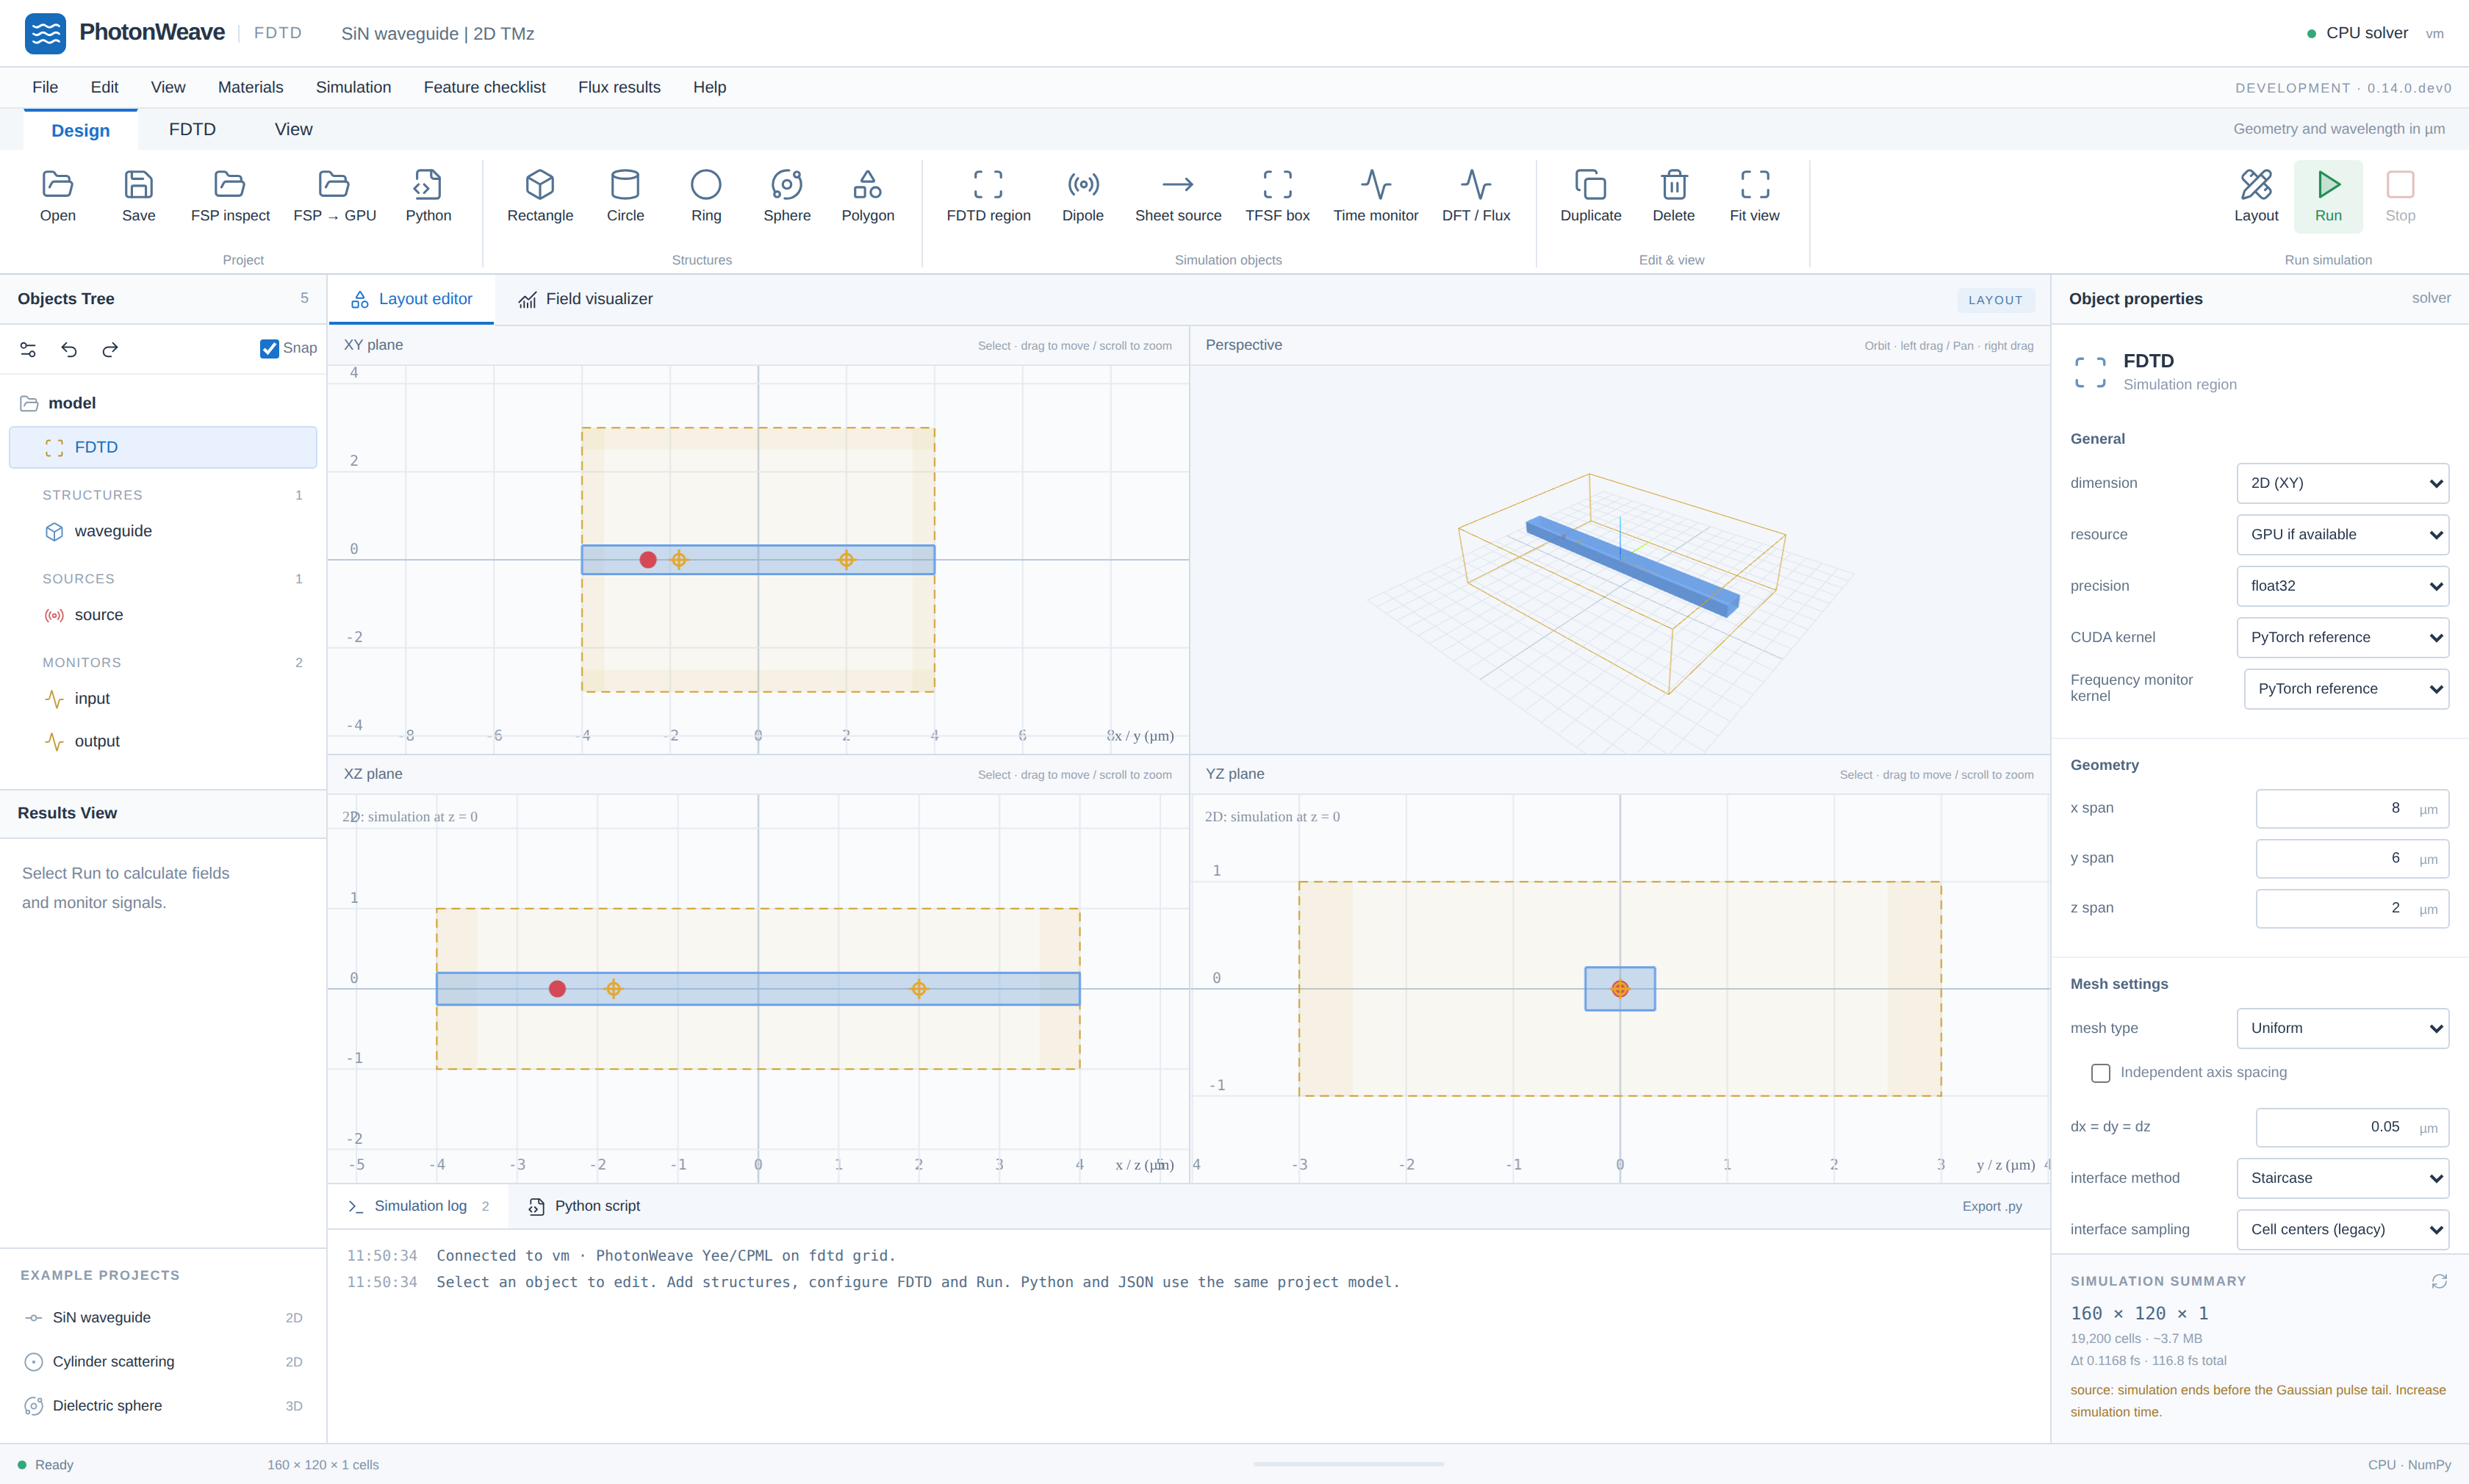
\includegraphics[width=.9\textwidth]{figures/ui-layout.png}\\[3pt]
    {\scriptsize\color{pwgrey} Hyoseok Park\quad·\quad 랩미팅 2026년 9월\quad·\quad 20분 버전 (상세 슬라이드는 부록)}
  \end{center}
\end{frame}}

% ------------------------------------------------------------- 2. summary --
\begin{frame}{한 장 요약}
  \begin{columns}[T]
    \begin{column}{.33\textwidth}
      \card{3.3cm}{6.5 -- 15.2$\times$}{Lumerical CPU(16 threads) 대비 기록된 wall time 비\\ \textcolor{pwred}{과거 빌드 · 동일정확도 아님}}
      \vspace{2.5mm}
      \card{3.3cm}{9.6 -- 17.1$\times$}{동일 격자·소스·모니터에서 오픈소스 GPU 기준선 대비}
    \end{column}
    \begin{column}{.33\textwidth}
      \card{3.3cm}{$\approx$ 40$\times$}{같은 4케이스 배치: NumPy CPU 47.04 s $\rightarrow$ CUDA 1.175 s}
      \vspace{2.5mm}
      \card{3.3cm}{46.7 / 85.9$\times$}{adjoint 기울기 1회: CPU 대비 GPU resident (FP32 / complex FP64)}
    \end{column}
    \begin{column}{.33\textwidth}
      \card{3.3cm}{54 GiB}{48 GB VRAM을 넘는 상태를 streaming으로 전진+역전파 완료}
      \vspace{2.5mm}
      \card{3.3cm}{4.4e-6}{박막 해석해 대비 $R+T-1$ 잔차 (오늘 CPU에서 재현)}
    \end{column}
  \end{columns}
  \vspace{2.5mm}
  \begin{center}
    \small 순서: \hl{왜 만들었나} $\rightarrow$ \hl{무엇을 만들었나} $\rightarrow$ \hl{정확도} $\rightarrow$ \hl{속도} $\rightarrow$ \hl{역설계} $\rightarrow$ \hl{한계}
  \end{center}
\end{frame}

% ------------------------------------------------------------ 3. why/what --
\begin{frame}{왜 직접 만들었나}
  \begin{columns}[T]
    \begin{column}{.95\textwidth}
      \begin{itemize}\footnotesize
        \item 스윕/역설계는 \hl{케이스 수만큼 순차 실행}, 동시 실행 개수는 보유 라이선스에 묶임.
              우리가 비교 기록을 가진 구성은 \hl{CPU 16 스레드 엔진}입니다 (상용 GPU 엔진은 미비교)
        \item 목적함수의 \hl{기울기}를 사용자 코드에서 받을 수 없어, 설계 루프가 사람의 판단 속도에 묶임
      \end{itemize}
    \end{column}
  \end{columns}
  \vspace{1mm}
  \begin{center}
      \begin{center}
        \begin{tikzpicture}[font=\scriptsize, scale=.72, every node/.style={transform shape},
          lay/.style={draw=pwgrey, fill=white, rounded corners=2pt, inner sep=4pt, text width=2.2cm, align=center, minimum height=8mm},
          new/.style={lay, draw=pwblue, fill=pwblue!8},
          lbl/.style={font=\scriptsize\bfseries, color=pwdeep}]
          \node[lbl, align=right] at (-.9,1.15) {기존};
          \node[lay] (a1) at (1.5,1.15) {GUI 구조 편집};
          \node[lay] (a2) at (4.3,1.15) {CPU 엔진\\1 케이스};
          \node[lay] (a3) at (7.1,1.15) {결과 파일};
          \node[lay] (a4) at (9.9,1.15) {사람이 판단};
          \draw[-Stealth, pwgrey] (a1)--(a2); \draw[-Stealth, pwgrey] (a2)--(a3); \draw[-Stealth, pwgrey] (a3)--(a4);
          \draw[-Stealth, pwgrey] (a4.north) to[out=90,in=90,looseness=.32] node[above, font=\tiny, color=pwgrey] {한 번에 한 구조} (a1.north);
          \node[lbl, align=right] at (-.9,-1.5) {PhotonWeave};
          \node[new] (b1) at (1.5,-1.5) {브라우저 CAD\\Python · FSP};
          \node[new] (b2) at (4.3,-1.5) {CUDA 네이티브\\$N$ 케이스 동시};
          \node[new] (b3) at (7.1,-1.5) {목적함수\\+ 기울기};
          \node[new] (b4) at (9.9,-1.5) {최적화기가\\자동 판단};
          \draw[-Stealth, pwblue] (b1)--(b2); \draw[-Stealth, pwblue] (b2)--(b3); \draw[-Stealth, pwblue] (b3)--(b4);
          \draw[-Stealth, pwblue] (b4.south) to[out=-90,in=-90,looseness=.32] node[below, font=\tiny, color=pwblue] {한 번에 설계 공간 전체} (b1.south);
        \end{tikzpicture}
      \end{center}
  \end{center}
  \vspace{-1mm}
  \begin{center}
    \small 바꾼 것: \hl{익숙한 UI}는 유지, 계산은 \hl{GPU 배치}로, 기울기는 \hl{discrete adjoint}로 노출.
  \end{center}
\end{frame}

% --------------------------------------------------------- 4. architecture --
\begin{frame}{시스템 구조}
  \begin{center}
    \begin{tikzpicture}[font=\scriptsize, scale=.88, every node/.style={transform shape},
      blk/.style={draw=pwgrey, fill=white, rounded corners=2pt, inner sep=5pt, align=center},
      hi/.style={blk, draw=pwblue, fill=pwblue!8},
      gpu/.style={blk, draw=pwgreen, fill=pwgreen!8}]
      \node[hi, text width=3.1cm] (ui) at (0,2.8) {\textbf{브라우저 워크벤치}\\Objects Tree · CAD 4뷰\\재료/메시/모니터 편집};
      \node[hi, text width=3.1cm] (py) at (4.2,2.8) {\textbf{Python API}\\\texttt{Project / Simulation}\\\texttt{BatchRunner / optimize}};
      \node[hi, text width=3.1cm] (fsp) at (8.4,2.8) {\textbf{FSP 브리지}\\독립 리더/라이터\\(.fsp 구조·설정 일부)};
      \node[blk, text width=11.2cm] (model) at (4.2,1.5) {\textbf{공통 프로젝트 모델} (JSON schema, µm 단위) — 구조 · 재료 · 소스 · 모니터 · 메시 · 경계};
      \node[blk, text width=11.2cm] (solver) at (4.2,0.3) {\textbf{솔버 코어} — Yee 업데이트 · 6면 CPML · 주기/Bloch · graded/rectilinear 메시 · ADE 분산재료};
      \node[gpu, text width=3.4cm] (torch) at (-0.1,-1.1) {PyTorch 경로\\CPU / CUDA, float32/64};
      \node[gpu, text width=3.4cm] (fused) at (4.2,-1.1) {fused CUDA 커널\\+ CUDA Graph};
      \node[gpu, text width=3.4cm] (adj) at (8.5,-1.1) {discrete adjoint\\+ checkpoint replay};
      \node[blk, text width=11.2cm, draw=pwamber, fill=pwamber!8] (mem) at (4.2,-2.3) {\textbf{메모리 계층} — VRAM resident / DRAM 스트리밍 / 파일 백킹 (space-time tile)};
      \draw[-Stealth, pwdeep] (ui)--(model); \draw[-Stealth, pwdeep] (py)--(model); \draw[-Stealth, pwdeep] (fsp)--(model);
      \draw[-Stealth, pwdeep] (model)--(solver);
      \draw[-Stealth, pwdeep] (solver)--(torch); \draw[-Stealth, pwdeep] (solver)--(fused); \draw[-Stealth, pwdeep] (solver)--(adj);
      \draw[-Stealth, pwdeep] (torch)--(mem); \draw[-Stealth, pwdeep] (fused)--(mem); \draw[-Stealth, pwdeep] (adj)--(mem);
    \end{tikzpicture}
  \end{center}
  \vspace{1mm}
  \caveat{그리드/백엔드 기반은 오픈소스 flaport/fdtd(MIT)를 사용하고, Yee 미분 · CPML · 주기/Bloch · CUDA Graph 실행은 직접 구현했습니다.}
\end{frame}

% ------------------------------------------------------------------ 5. UI --
\begin{frame}{익숙한 워크플로: Layout $\rightarrow$ Run $\rightarrow$ Analysis}
  \begin{columns}[T]
    \begin{column}{.49\textwidth}
      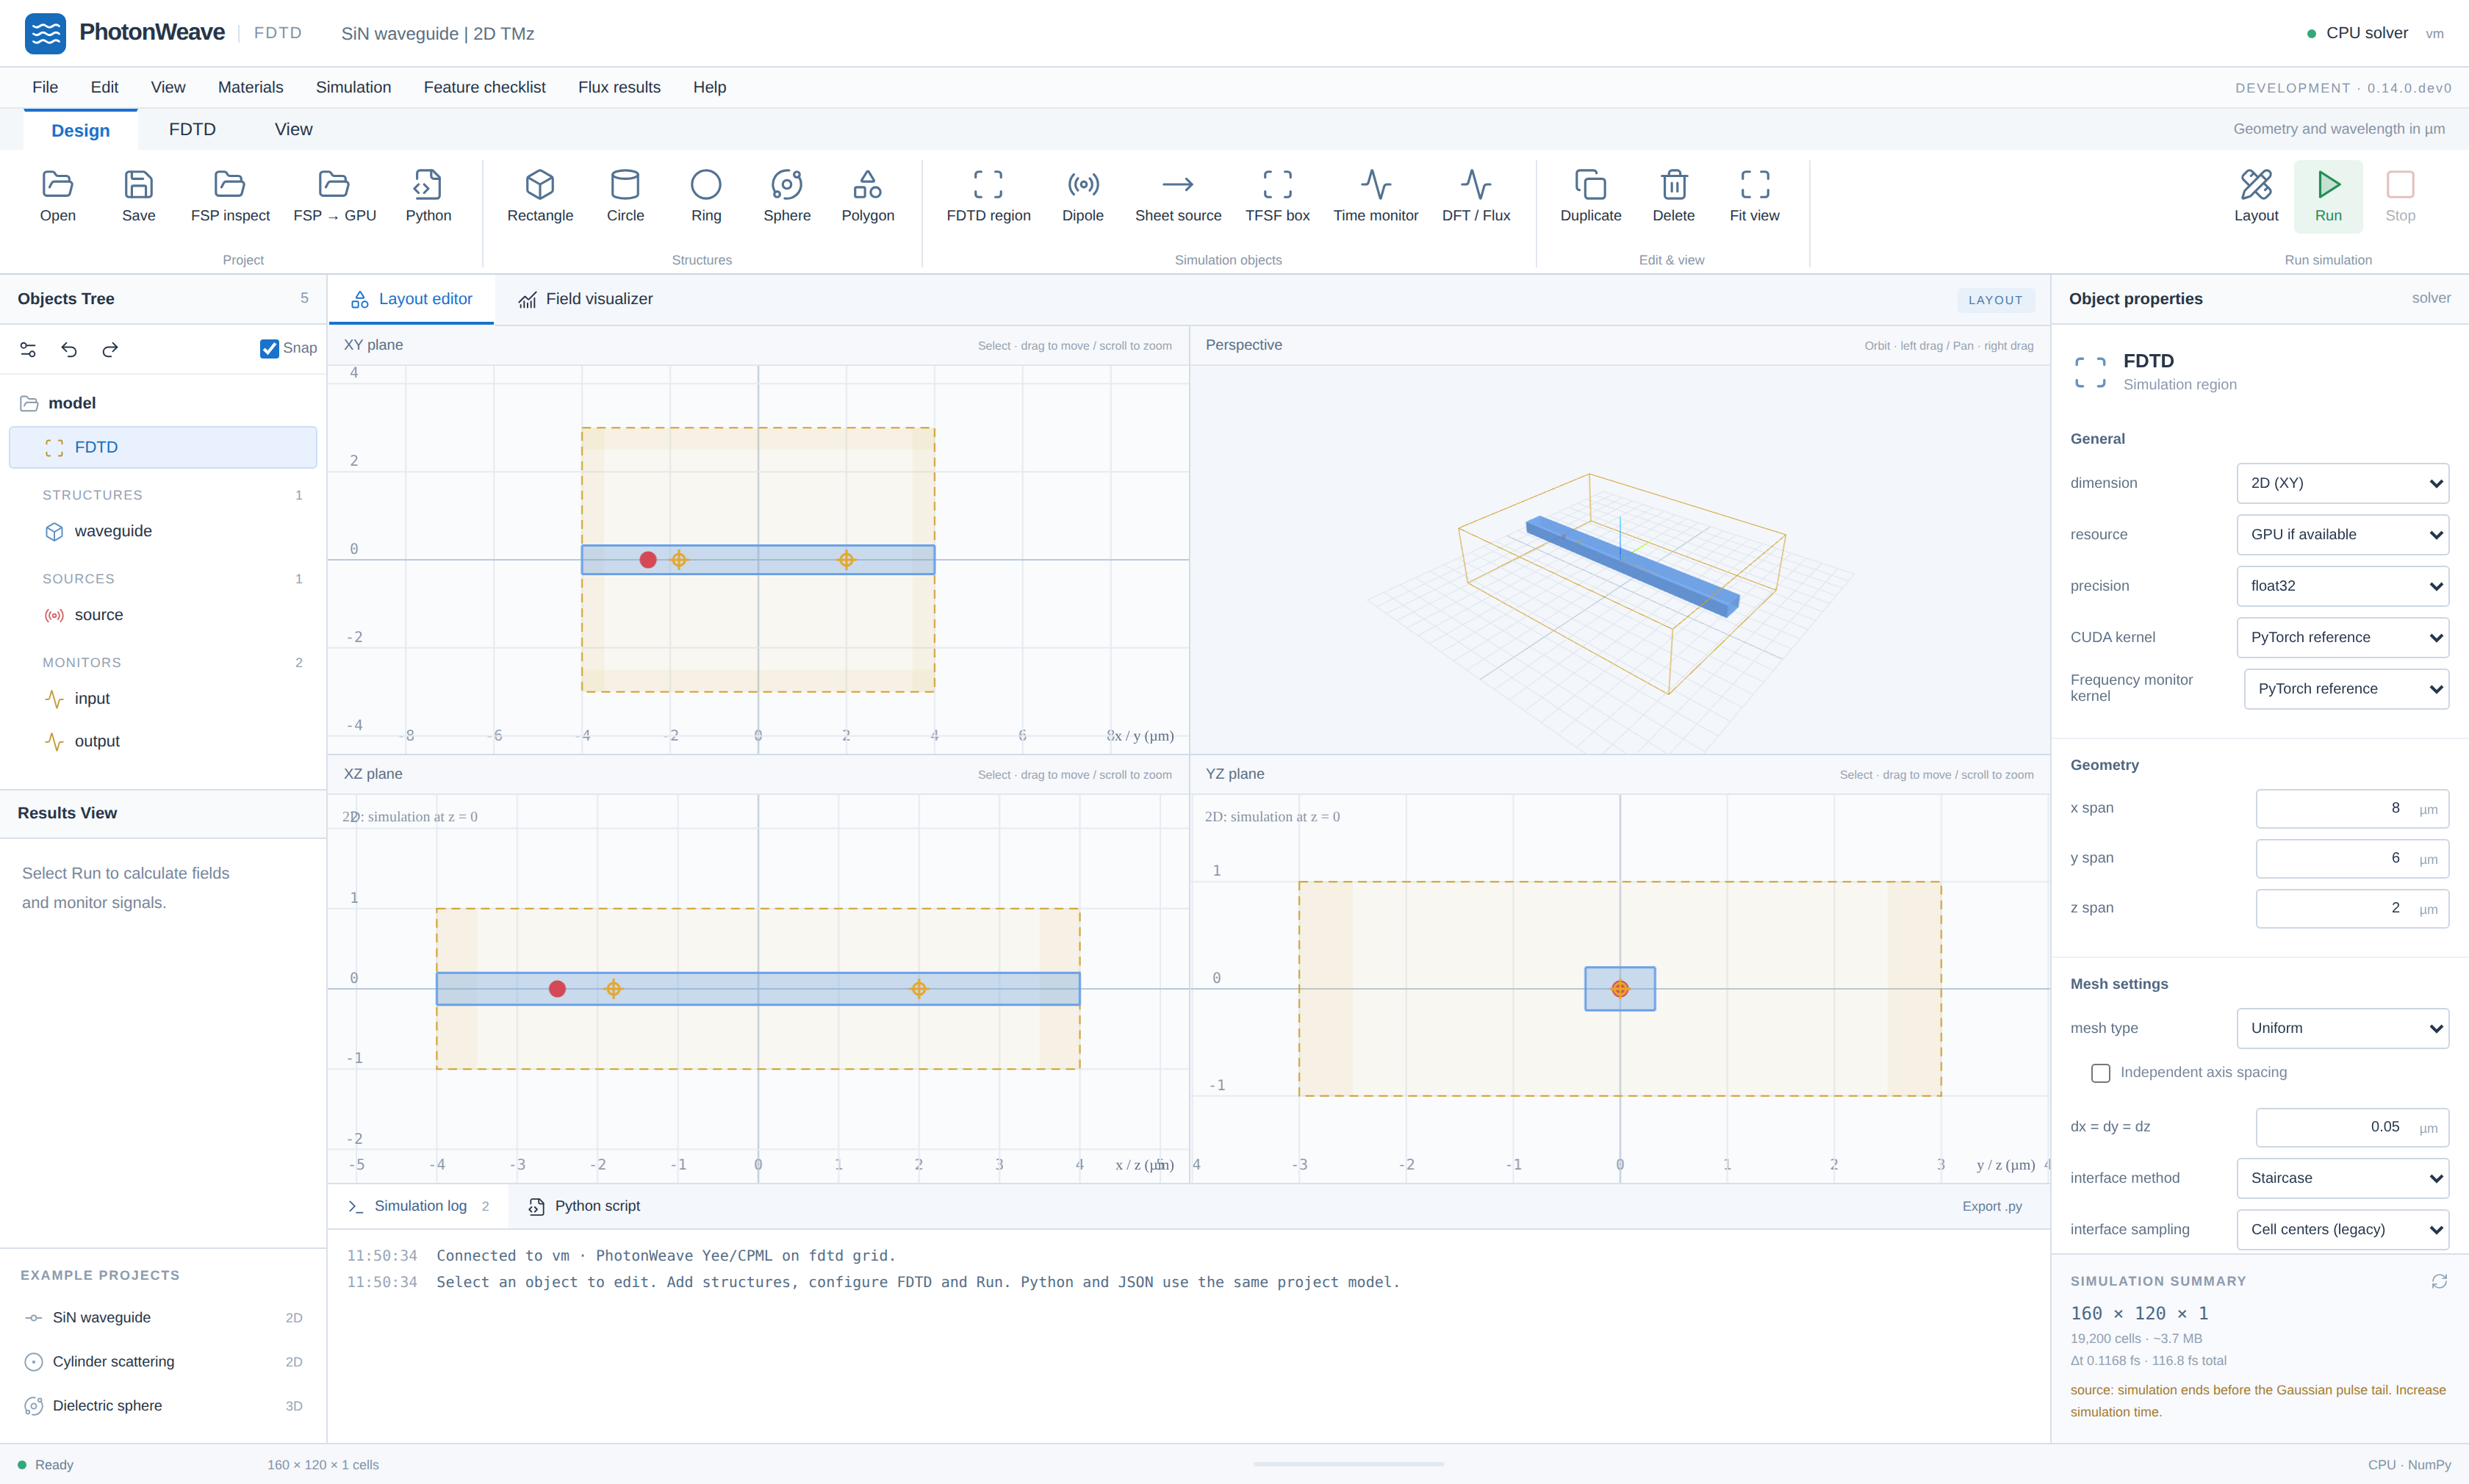
\includegraphics[width=\textwidth]{figures/ui-layout.png}\\[1mm]
      \caveat{구조 트리 · CAD 4뷰 · 객체 속성 · 재료/메시 설정}
    \end{column}
    \begin{column}{.49\textwidth}
      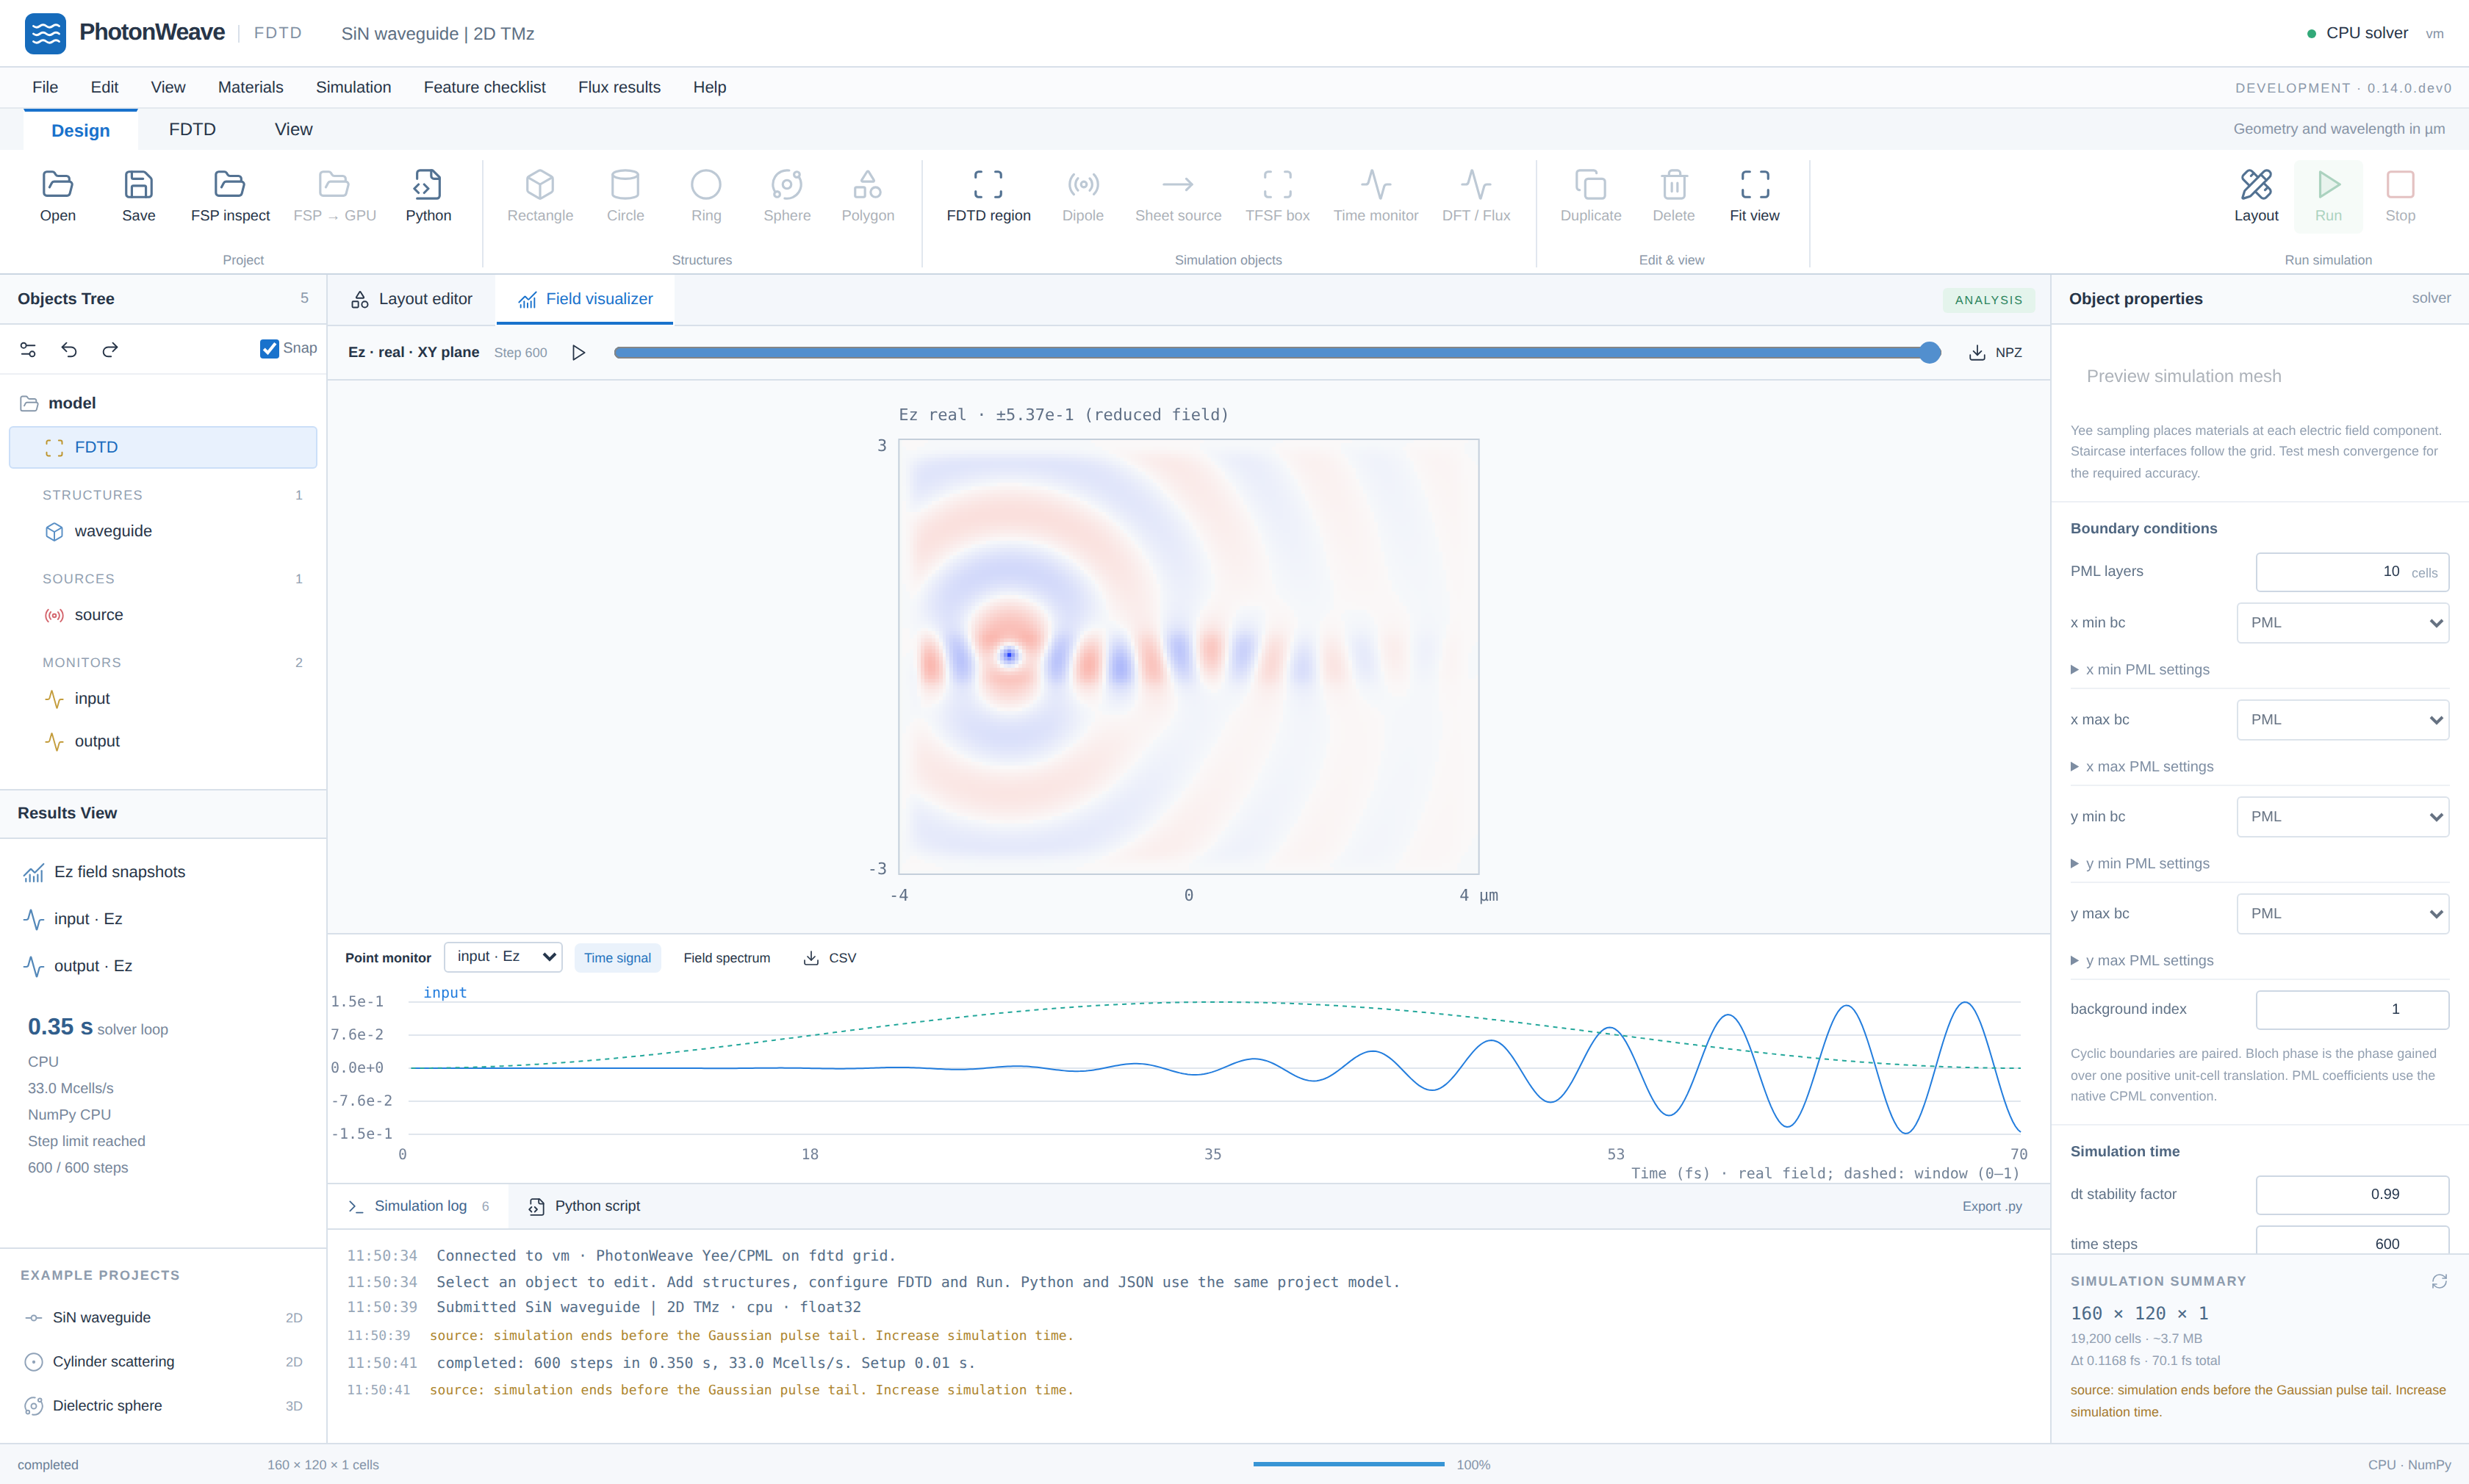
\includegraphics[width=\textwidth]{figures/ui-results.png}\\[1mm]
      \caveat{필드 스냅샷 애니메이션 · 모니터 시계열/스펙트럼 · NPZ/CSV · Python export}
    \end{column}
  \end{columns}
  \vspace{2mm}
  \begin{center}
    \small 브라우저에서 만든 구조가 \hl{그대로 Python 객체}입니다. UI $\rightarrow$ JSON $\rightarrow$ 스크립트가 같은 모델.
  \end{center}
\end{frame}

% -------------------------------------------------------------- 6. engine --
\begin{frame}{엔진: Yee/CPML을 직접 구현하고 CUDA로 융합}
  \begin{columns}[T]
    \begin{column}{.44\textwidth}
      \begin{center}
        \begin{tikzpicture}[x={(1.05cm,0cm)}, y={(0cm,1.05cm)}, z={(-0.52cm,-0.40cm)},
                            font=\scriptsize, line join=round]
          \foreach \dx in {0, 2.2} {
            \begin{scope}[xshift=\dx cm]
              \draw[pwgrey!75] (0,0,0)--(1,0,0)--(1,1,0)--(0,1,0)--cycle;
              \draw[pwgrey!35] (0,0,1)--(1,0,1)--(1,1,1)--(0,1,1)--cycle;
              \draw[pwgrey!35] (0,0,0)--(0,0,1); \draw[pwgrey!35] (1,0,0)--(1,0,1);
              \draw[pwgrey!35] (1,1,0)--(1,1,1); \draw[pwgrey!35] (0,1,0)--(0,1,1);
            \end{scope}}
          \draw[-Stealth, pwblue, very thick] (0,0,0)--(.7,0,0);
          \node[pwblue, anchor=north] at (.5,0,0) {$E_x$};
          \draw[-Stealth, pwblue, very thick] (0,0,0)--(0,.7,0);
          \node[pwblue, anchor=east] at (0,.55,0) {$E_y$};
          \draw[-Stealth, pwblue, very thick] (0,0,0)--(0,0,.7);
          \node[pwblue, anchor=south east] at (0,0,.6) {$E_z$};
          \fill[pwdeep] (0,0,0) circle (1.1pt);
          \node[anchor=north, font=\scriptsize] at (.5,-.34,0) {$\mathbf{E}$: 모서리};
          \begin{scope}[xshift=2.4cm]
            \draw[-Stealth, pwred, very thick] (1,.5,.5)--(1.5,.5,.5);
            \node[pwred, anchor=west] at (1.5,.5,.5) {$H_x$};
            \draw[-Stealth, pwred, very thick] (.5,1,.5)--(.5,1.45,.5);
            \node[pwred, anchor=south] at (.5,1.45,.5) {$H_y$};
            \draw[-Stealth, pwred, very thick] (.5,.5,1)--(.5,.5,1.5);
            \node[pwred, anchor=east] at (.5,.5,1.5) {$H_z$};
            \fill[pwred!70] (1,.5,.5) circle (1.1pt);
            \fill[pwred!70] (.5,1,.5) circle (1.1pt);
            \fill[pwred!70] (.5,.5,1) circle (1.1pt);
            \node[anchor=north, font=\scriptsize] at (.5,-.34,0) {$\mathbf{H}$: 면 중심};
          \end{scope}
        \end{tikzpicture}
      \end{center}
      \vspace{1mm}
      \caveat{3D 6성분 + 2D TMz/TEz, float32/64, 실수장과 복소장(Bloch), CFL 기본 0.99.}
    \end{column}
    \begin{column}{.54\textwidth}
      \begin{itemize}\footnotesize
        \item \hl{경계}: 면별 독립 CPML(3D 6면) + 주기/Bloch 쌍 \\ \textcolor{pwred}{대칭/PEC/PMC는 미구현}
        \item \hl{소스}: 점 dipole, soft sheet, one-way 주기 평면, closed TFSF box (수직 입사)
        \item \hl{메시}: uniform / graded / 축별 독립 rectilinear, 직사각형 CFL
        \item \hl{재료}: 상수 $n$ + 수동 Drude/Lorentz 최대 16 극점, 측정 n/k 피팅
        \item \hl{실행}: fused Yee/CPML CUDA 커널 + CUDA Graph + \textbf{케이스 배치 축}
      \end{itemize}
      \vspace{1mm}
      \begin{block}{\footnotesize 배치 축이 핵심}
        \footnotesize 독립 구조 $N$개를 한 번의 커널 launch로 전진시키고, 결과는 개별 실행과 \hl{bitwise 동일}합니다.
      \end{block}
    \end{column}
  \end{columns}
\end{frame}

% ------------------------------------------------------------ 7. accuracy --
\begin{frame}{정확도: 해석해와 비교}
  \vspace{2mm}
  \begin{columns}[T]
    \begin{column}{.58\textwidth}
      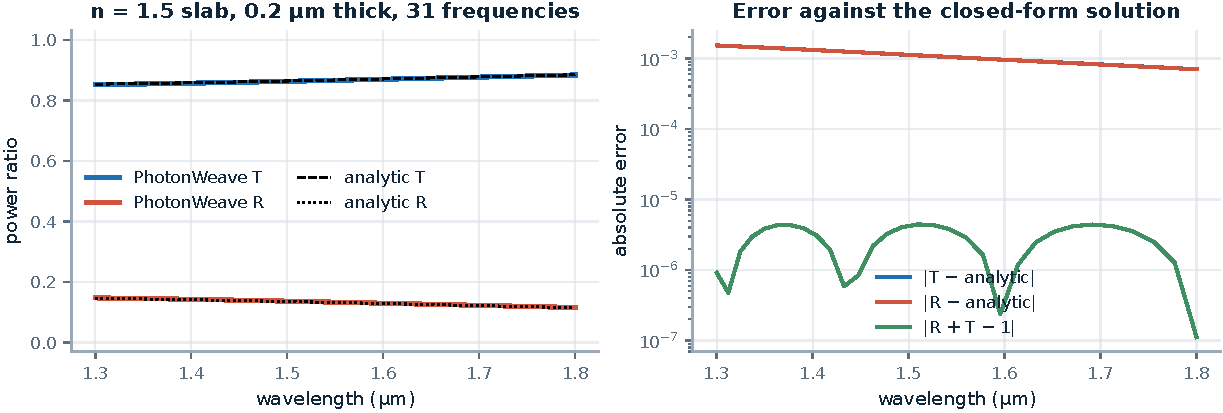
\includegraphics[width=\textwidth]{figures/field-slab-validation.pdf}\\[1mm]
      \caveat{$n=1.5$ 박막: 최대 오차 $|T-T_\text{exact}|=$ \num{1.53e-3}, 에너지 잔차 \num{4.44e-6}. 오늘 CPU float64로 1.4초 만에 재현.}
    \end{column}
    \begin{column}{.40\textwidth}
      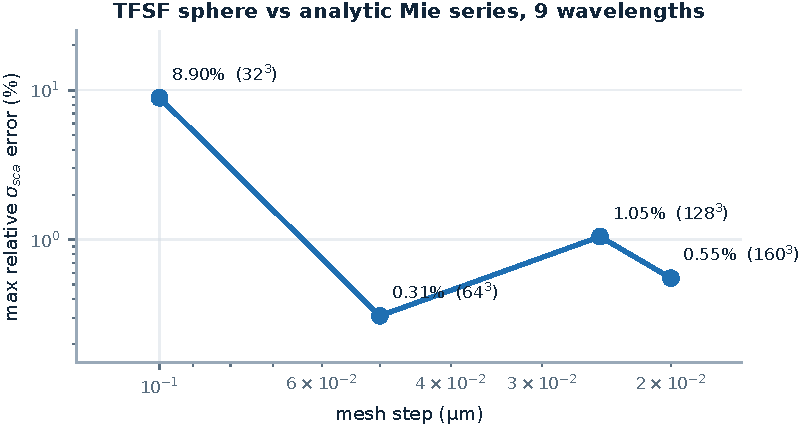
\includegraphics[width=\textwidth]{figures/chart-mie.pdf}\\[1mm]
      \caveat{TFSF 구 산란 대 Mie 급수. 0.05 µm에서 0.31\%지만 \alert{오차가 단조 감소하지 않습니다} — 정량 결과에는 수렴 테스트 필요.}
    \end{column}
  \end{columns}
\end{frame}

% ---------------------------------------------------------------- 8. PhC ---
\begin{frame}{우리 연구 대상으로 직접 계산: 밴드갭과 W1 도파로}
  \begin{columns}[T]
    \begin{column}{.55\textwidth}
      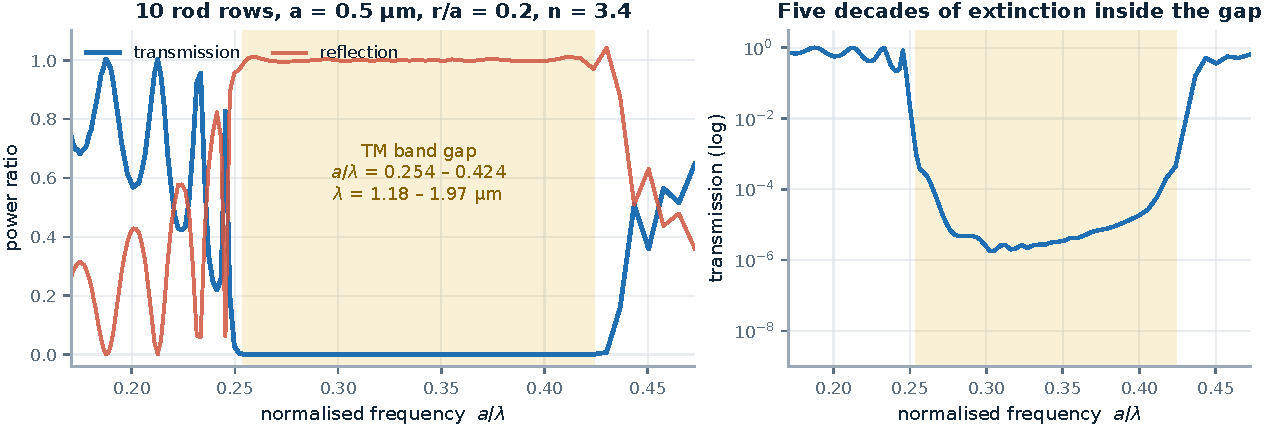
\includegraphics[width=\textwidth]{figures/field-phc-gap.pdf}\\[1mm]
      \caveat{정사각 rod 격자 ($a=0.5$ µm, $r/a=0.2$, $n=3.4$) 10열, broadband one-way 평면 소스 + 주기 경계 + flux 모니터. CPU에서 약 30초.}
    \end{column}
    \begin{column}{.43\textwidth}
      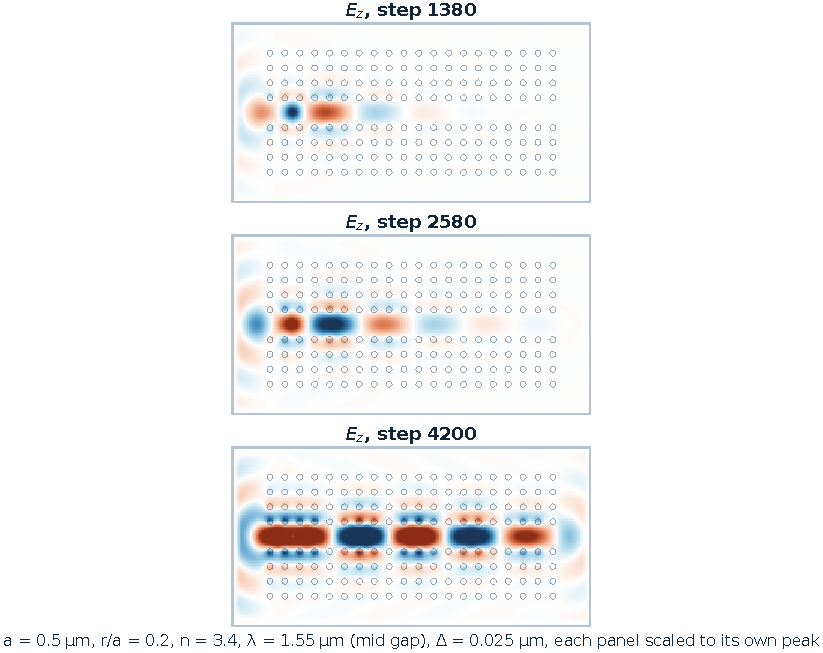
\includegraphics[width=\textwidth]{figures/field-phc-w1.pdf}\\[1mm]
      \caveat{같은 결정의 W1 선결함을 밴드갭 안쪽 1.55 µm로 여기. 결정 안쪽은 evanescent, 채널을 따라 전파. 160 rod / 6000 스텝 / CPU 22초.}
    \end{column}
  \end{columns}
\end{frame}

% ----------------------------------------------------------- 9. Lumerical --
\begin{frame}{속도 1: Lumerical FDTD와의 기록된 비교}
  \begin{center}
    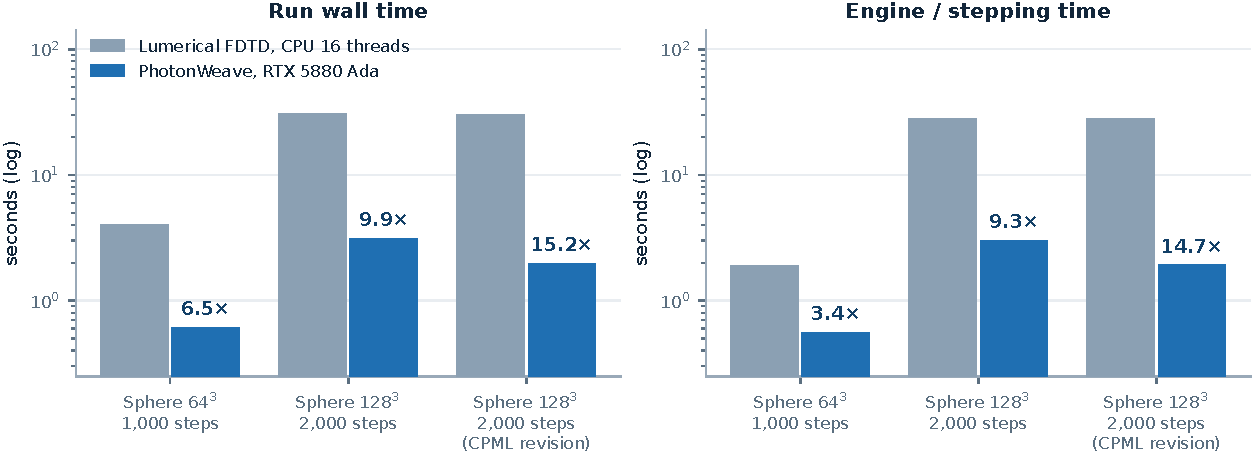
\includegraphics[width=.88\textwidth]{figures/chart-lumerical.pdf}
  \end{center}
  \vspace{-2mm}
  \begin{columns}[T]
    \begin{column}{.5\textwidth}
      \footnotesize 6 µm 도메인의 $n=2$ 구, 1.55 µm Gaussian dipole, 포인트 모니터 1개, 3회 측정의 중앙값.
    \end{column}
    \begin{column}{.47\textwidth}
      \begin{block}{\footnotesize 이 표를 읽는 법}
        \scriptsize \textcolor{pwred}{과거 빌드의 기록}이며 현재 릴리스의 검증된 speedup이 아닙니다.
        dipole 정규화·필드 보간·흡수 경계가 달라 \textcolor{pwred}{동일 정확도 비교가 아니고}, Lumerical GPU 엔진과는 측정하지 않았습니다.
      \end{block}
    \end{column}
  \end{columns}
\end{frame}

% ------------------------------------------------------------ 10. GPU/CPU --
\begin{frame}{속도 2: 같은 물리 설정에서 측정한 것}
  \begin{columns}[T]
    \begin{column}{.56\textwidth}
      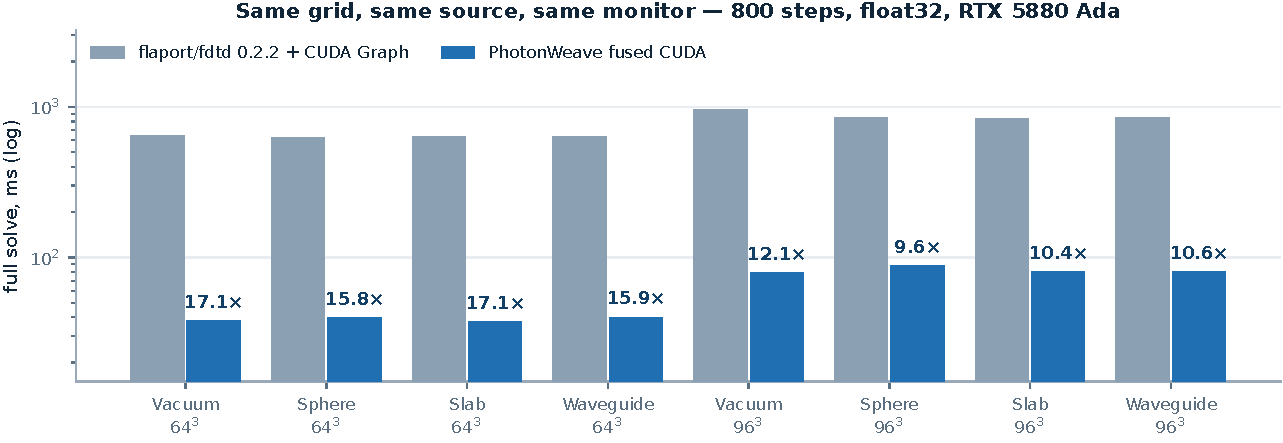
\includegraphics[width=\textwidth]{figures/chart-flaport.pdf}\\[1mm]
      \caveat{두 엔진에 동일한 voxel 유전율·시간 스텝·소스·모니터를 주고, 공개 코드에 CUDA Graph 어댑터까지 붙여 준 비교. 포인트 트레이스 상대 L2 $<$0.04\%.}
    \end{column}
    \begin{column}{.42\textwidth}
      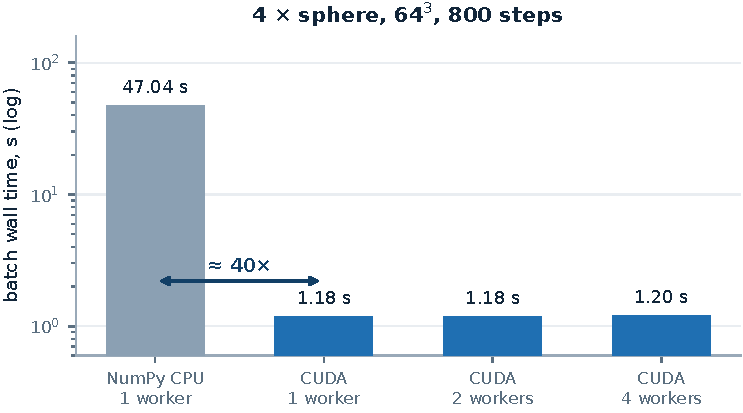
\includegraphics[width=\textwidth]{figures/chart-cpu-gpu.pdf}\\[1mm]
      \caveat{4개 독립 구 케이스, 64$^3$, 800 스텝. 워커를 2/4개로 늘려도 이 문제에서는 더 빨라지지 않습니다.}
      \vspace{1mm}
      {\footnotesize 배치 축은 32$^3$에서 \num{112 cases/s}까지 오르지만, 64$^3$의 8/16 케이스에서는 \alert{오히려 느려집니다} (부록).}
    \end{column}
  \end{columns}
\end{frame}

% ------------------------------------------------------------ 11. ablation --
\begin{frame}{속도 3: 시간이 실제로 줄어든 곳}
  \begin{center}
    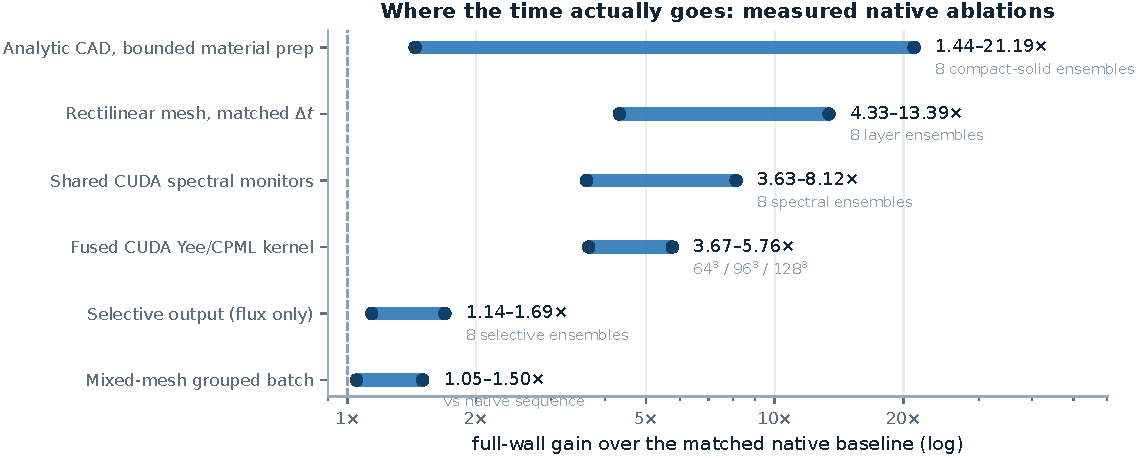
\includegraphics[width=.86\textwidth]{figures/chart-ablation.pdf}
  \end{center}
  \vspace{-1mm}
  \footnotesize
  단일 커널 최적화만이 아니라 \hl{호스트 준비 시간 · 불필요한 셀 · 저장하지 않아도 되는 출력}을 제거한 것이
  워크플로 시간에 더 크게 기여했습니다. 모든 행은 동일 조건의 네이티브 baseline과 비교한 full-wall 시간입니다.
\end{frame}

% ------------------------------------------------------------- 12. adjoint --
\begin{frame}{역설계: discrete adjoint로 기울기를 직접 계산}
  \begin{columns}[T]
    \begin{column}{.45\textwidth}
      \begin{center}
        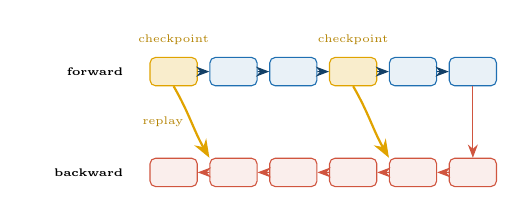
\begin{tikzpicture}[font=\tiny, scale=.8, every node/.style={transform shape},
          st/.style={draw=pwblue, fill=pwblue!10, rounded corners=2pt, minimum width=.75cm, minimum height=.45cm},
          ck/.style={draw=pwamber, fill=pwamber!20, rounded corners=2pt, minimum width=.75cm, minimum height=.45cm},
          ad/.style={draw=pwred, fill=pwred!10, rounded corners=2pt, minimum width=.75cm, minimum height=.45cm}]
          \node[align=right, text width=1.4cm] at (-1.5,.8) {\textbf{forward}};
          \foreach \i in {0,...,5} {
            \ifnum\i=0 \node[ck] (f\i) at (\i*.95,.8) {};
            \else\ifnum\i=3 \node[ck] (f\i) at (\i*.95,.8) {};
            \else \node[st] (f\i) at (\i*.95,.8) {}; \fi\fi}
          \foreach \i [evaluate=\i as \j using int(\i+1)] in {0,...,4} \draw[-Stealth, pwdeep] (f\i)--(f\j);
          \node[align=right, text width=1.4cm] at (-1.5,-.8) {\textbf{backward}};
          \foreach \i in {0,...,5} \node[ad] (b\i) at (\i*.95,-.8) {};
          \foreach \i [evaluate=\i as \j using int(\i+1)] in {0,...,4} \draw[Stealth-, pwred] (b\i)--(b\j);
          \draw[-Stealth, pwred] (f5.south)--(b5.north);
          \draw[-Stealth, pwamber, thick] (f0.south) to[out=-60,in=120] node[left, pwamber!80!black] {replay} (b1.north west);
          \draw[-Stealth, pwamber, thick] (f3.south) to[out=-60,in=120] (b4.north west);
          \node[pwamber!80!black, above] at (0,1.1) {checkpoint};
          \node[pwamber!80!black, above] at (2.85,1.1) {checkpoint};
        \end{tikzpicture}
      \end{center}
      \vspace{1mm}
      \begin{itemize}\footnotesize
        \item 파라미터가 $P$개여도 기울기 1회 = forward 1회 + backward 1회 (유한차분은 $P+1$회)
        \item 전체 시간 이력 대신 \hl{checkpoint replay}로 메모리 제한
        \item 대각 $\varepsilon$, Torch geometry, Drude/Lorentz 파라미터까지 미분
      \end{itemize}
    \end{column}
    \begin{column}{.53\textwidth}
      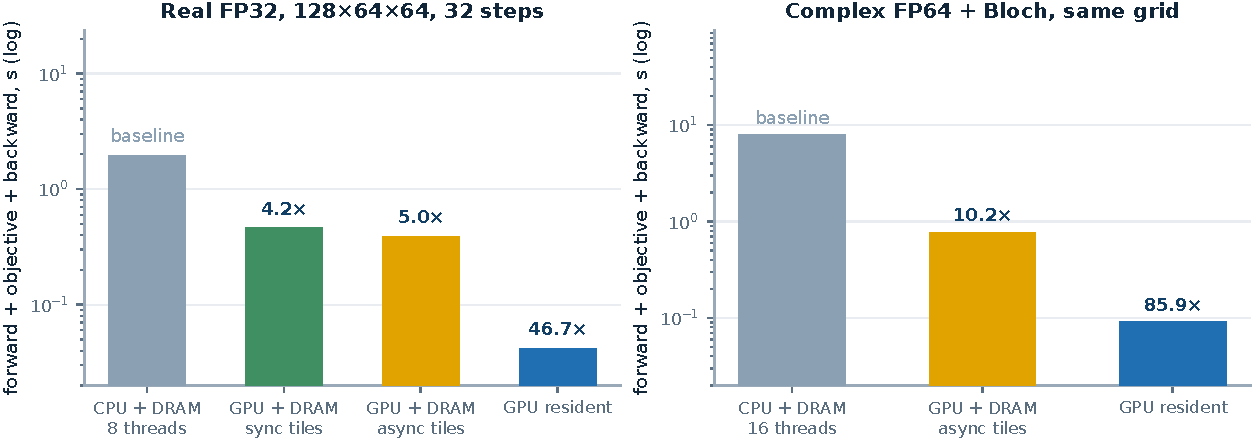
\includegraphics[width=\textwidth]{figures/chart-adjoint.pdf}\\[1mm]
      \caveat{같은 코드 경로·같은 격자(128$\times$64$\times$64, 32 스텝)의 forward + 목적함수 + backward 전체 시간. 모든 모드가 신호·기울기 검사를 통과, CPU는 최적 스레드 수 사용. 이 문제는 VRAM 안에 들어갑니다.}
    \end{column}
  \end{columns}
\end{frame}

% -------------------------------------------------------------- 13. memory --
\begin{frame}{VRAM보다 큰 문제도 푼다}
  \begin{columns}[T]
    \begin{column}{.45\textwidth}
      \begin{center}
        \begin{tikzpicture}[font=\scriptsize, scale=.92, every node/.style={transform shape},
          tier/.style={draw=pwgrey, rounded corners=2pt, minimum width=4.4cm, minimum height=.9cm, align=center}]
          \node[tier, fill=pwblue!12, draw=pwblue] (v) at (0,2.0) {\textbf{VRAM (48 GB)}\\현재 타일 + 실행 버퍼};
          \node[tier, fill=pwgreen!10, draw=pwgreen] (d) at (0,.8) {\textbf{DRAM 뱅크}\\전체 E/H · ADE 상태};
          \node[tier, fill=pwamber!12, draw=pwamber] (f) at (0,-.4) {\textbf{파일 백킹 (NVMe)}\\더 큰 상태, 실험적};
          \draw[-Stealth, pwdeep] (v.west) to[out=180, in=180] node[left, font=\tiny] {tile out} (d.west);
          \draw[-Stealth, pwdeep] (d.east) to[out=0, in=0] node[right, font=\tiny] {tile in} (v.east);
          \draw[-Stealth, pwgrey] (d.south)--(f.north);
          \node[align=center, font=\tiny, text width=5cm] at (0,-1.4) {space-time tile: 한 칸 Yee 의존 cone을\\halo로 포함해 손실 없이 분할};
        \end{tikzpicture}
      \end{center}
    \end{column}
    \begin{column}{.52\textwidth}
      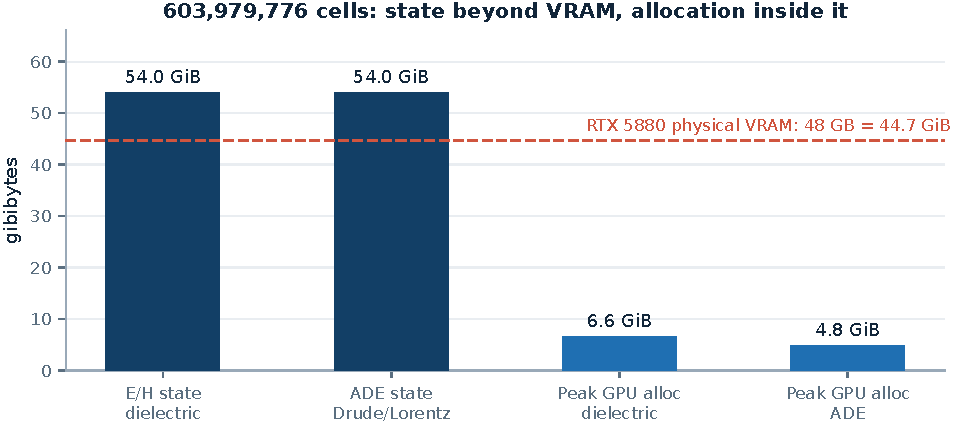
\includegraphics[width=\textwidth]{figures/chart-beyond-vram.pdf}\\[1mm]
      \footnotesize
      603,979,776 셀, E/H 54 GiB 상태에서 \hl{10 스텝 전진 + 1차 기울기} 검증 완료
      (peak GPU 할당 6.6 GiB, 52분).
      \caveat{용량 증명이지 속도 우위가 아닙니다. 실제 응용 지속시간에서의 성능은 미검증.}
    \end{column}
  \end{columns}
\end{frame}

% -------------------------------------------------------------- 14. limits --
\begin{frame}{아직 안 되는 것과 다음 단계}
  \begin{columns}[T]
    \begin{column}{.48\textwidth}
      \textbf{\small 한계}
      \begin{itemize}\footnotesize
        \item 이득 매질 · 비선형 · 이방성 미지원, 대칭/PEC/PMC 미구현
        \item 경사 입사 one-way/TFSF, 도파로 모드 소스, far-field, mode port 미구현
        \item 체크리스트 1,661행 중 구현 160 / 부분 231 \caveat{(속성 수, 완성도 비율 아님)}
        \item 상용 솔버와 \alert{동일 정확도 조건의 재측정}이 아직 남아 있음
      \end{itemize}
    \end{column}
    \begin{column}{.48\textwidth}
      \textbf{\small 다음 단계}
      \begin{itemize}\footnotesize
        \item 공통 정확도 목표로 상용 솔버 재측정, Lumerical GPU 엔진 포함
        \item mode/port 정규화 목적함수 $\rightarrow$ 실제 역설계 검증
        \item 통합 메모리 정책 (resident/streamed 자동 선택)
        \item 랩 적용: PhC/metasurface 스윕을 배치로 이전, GPU 워크스테이션 공유
      \end{itemize}
    \end{column}
  \end{columns}
  \vspace{2mm}
  \begin{center}
    \small 필요한 구조·조건을 알려주시면 그 케이스로 먼저 벤치마크하고, 정확도 게이트를 붙여서 가져오겠습니다.
  \end{center}
\end{frame}

% --------------------------------------------------------------- 15. close --
\begin{frame}[standout]
  요약\\[4mm]
  {\normalsize
  \begin{minipage}{.8\textwidth}
    \begin{itemize}
      \item 상용 FDTD와 같은 작업 순서를 유지한 \textbf{브라우저 + Python 워크벤치}
      \item 같은 물리 설정에서 우리 CPU 경로와 공개 GPU 기준선보다 \textbf{빠른 CUDA 엔진}
      \item 설계 루프를 위한 \textbf{배치 실행과 discrete adjoint}, VRAM을 넘는 메모리 계층
      \item 속도 수치는 조건과 한계를 함께 기록 — 상용 솔버 동일정확도 비교는 \textbf{진행 중}
    \end{itemize}
  \end{minipage}}
\end{frame}

% ===========================================================================
\appendix

\begin{frame}{부록: 그래서 지금 다시 해야 하는 비교}
  \begin{center}\small
    \begin{tabular}{p{7.4cm} l}
      \toprule
      \textbf{필요한 비교} & \textbf{현재 상태} \\
      \midrule
      현재 PhotonWeave vs Lumerical CPU, 공통 정확도 목표 & \textcolor{pwred}{새 matched validation 필요} \\
      현재 PhotonWeave vs Lumerical GPU, 같은 RTX 5880 & \textcolor{pwred}{미측정} \\
      다구조 배치 / 역설계 throughput vs Lumerical & \textcolor{pwred}{미측정} \\
      \midrule
      오픈소스 GPU 기준선(flaport/fdtd + CUDA Graph) 대비 & \textcolor{pwgreen}{측정 완료} \\
      네이티브 CPU vs GPU, 동일 코드 경로 & \textcolor{pwgreen}{측정 완료} \\
      해석해(박막, Mie) 대비 정확도 & \textcolor{pwgreen}{측정 완료, 한계 명시} \\
      \bottomrule
    \end{tabular}
  \end{center}
  \vspace{2mm}
  \footnotesize 랩미팅에서 주장하는 범위: \hl{"같은 물리 설정에서 우리 GPU 경로가 우리 CPU 경로와 공개 GPU 기준선보다 빠르다"}.
\end{frame}

\begin{frame}{부록: 배치 축의 한계}
  \begin{columns}[T]
    \begin{column}{.5\textwidth}
      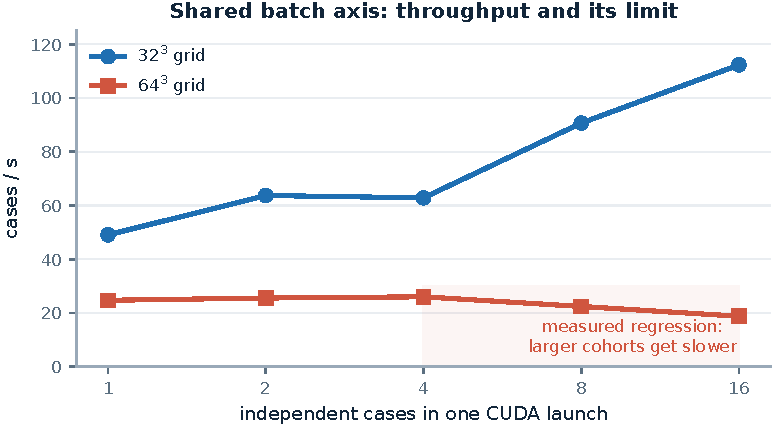
\includegraphics[width=\textwidth]{figures/chart-batch-scaling.pdf}
    \end{column}
    \begin{column}{.46\textwidth}
      \begin{itemize}\footnotesize
        \item 32$^3$에서는 16 케이스까지 throughput 증가 (\num{112 cases/s})
        \item 64$^3$에서는 8, 16 케이스에서 \alert{오히려 느려짐}
        \item \texttt{cohort\_size}로 한 번에 묶는 케이스 수를 제한
        \item \texttt{tune\_tensor\_batch()}가 측정으로 크기를 고르지만 \hl{튜닝 자체가 비용} (64$^3$에서 회수에 144--420 앙상블)
      \end{itemize}
      \source{README.md · ensembles.json}
    \end{column}
  \end{columns}
\end{frame}

\begin{frame}{부록: 혼합 메시 배치와 설계 루프}
  \begin{columns}[T]
    \begin{column}{.5\textwidth}
      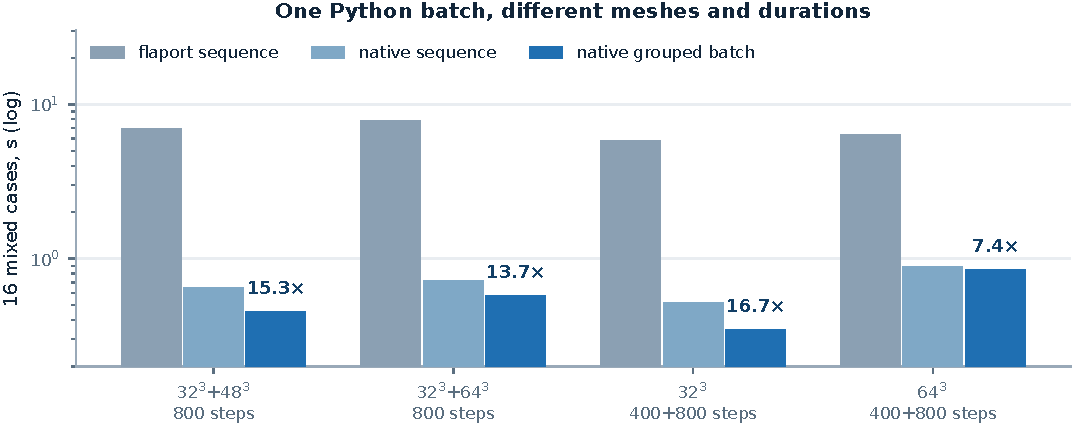
\includegraphics[width=\textwidth]{figures/chart-grouped.pdf}\\[1mm]
      \caveat{메시와 지속시간이 섞인 16 케이스를 한 Python 배치로. 호환 케이스를 자동 그룹화하고 입력 순서로 결과를 복원합니다.}
    \end{column}
    \begin{column}{.46\textwidth}
      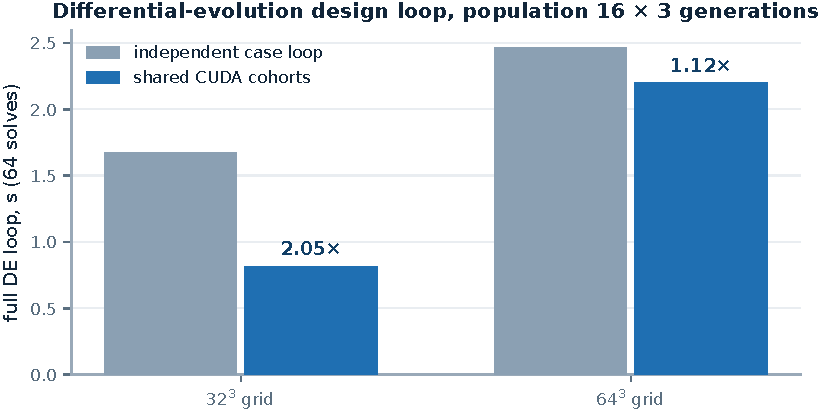
\includegraphics[width=\textwidth]{figures/chart-design-loop.pdf}\\[1mm]
      \caveat{블랙박스(미분 없는) differential evolution 루프, population 16 $\times$ 3세대 = 64회 forward.}
    \end{column}
  \end{columns}
\end{frame}

\begin{frame}{부록: 분산 재료(Drude/Lorentz) adjoint}
  \begin{center}
    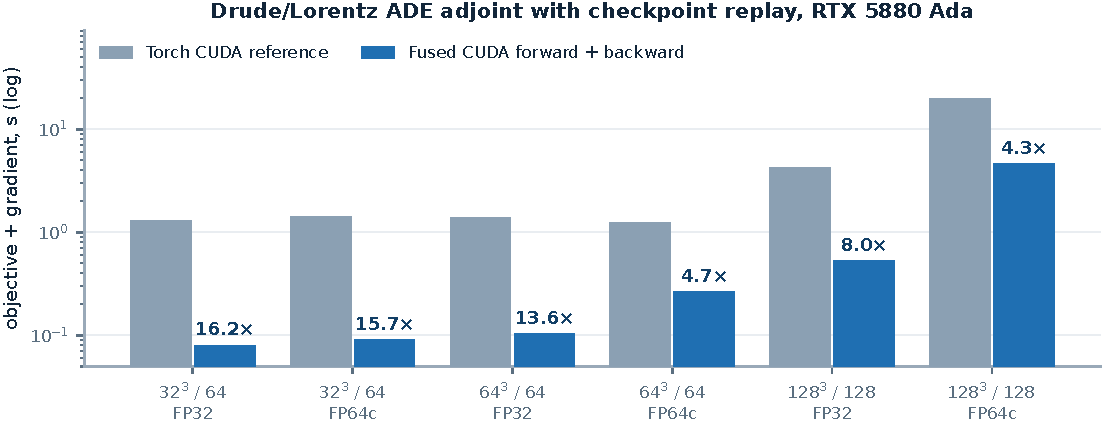
\includegraphics[width=.88\textwidth]{figures/chart-dispersive.pdf}
  \end{center}
  \vspace{-1mm}
  \footnotesize
  ADE의 P/Q 상태까지 checkpoint replay에 포함하고, 재료 기울기는 atomics 없이 블록 리덕션으로 모읍니다.
  공유 파라미터는 compact하게 유지되어 극점 수가 늘어도 메모리가 선형 증가하지 않습니다.
  \caveat{같은 연산(전진 + 목적함수 + 역전파)을 우리 Torch 경로와 비교한 내부 측정입니다.}
\end{frame}

\begin{frame}[fragile]{부록: 설계 루프 코드}
  \begin{columns}[T]
    \begin{column}{.55\textwidth}
\begin{lstlisting}[basicstyle=\ttfamily\tiny]
import torch
from photonweave import (DifferentiableSimulation,
    AdjointOptions, smooth_sphere_epsilon)

model = DifferentiableSimulation(project,
    AdjointOptions(checkpoints=4, storage="host"))
radius = torch.nn.Parameter(
    torch.tensor(0.25, dtype=torch.float64))
opt = torch.optim.Adam([radius], lr=0.003)

for step in range(iterations):
    opt.zero_grad()
    epsilon = smooth_sphere_epsilon(
        project.region, radius, width=0.09, inside=3.0)
    result = model(epsilon)             # forward
    loss = result.signals[:, 0].abs().square().mean()
    loss.backward()                     # discrete adjoint
    opt.step()
\end{lstlisting}
    \end{column}
    \begin{column}{.42\textwidth}
      \footnotesize
      \texttt{examples/differentiable\_design.py}의 실제 코드입니다.
      스트리밍 실행은 \texttt{StreamedSimulation}이 같은 자리에 들어갑니다.
      \vspace{2mm}
      \caveat{포트 정규화된 모드 목적함수와 응용 수준 역설계 검증은 진행 중입니다.}
    \end{column}
  \end{columns}
\end{frame}

\begin{frame}{부록: 기존 .fsp 자산과 오픈소스 지형}
  \begin{columns}[T]
    \begin{column}{.46\textwidth}
      \footnotesize
      \textbf{FSP 브리지}
      \begin{itemize}\footnotesize
        \item 벤더 런타임 없이 독립 파싱: box, 회전 타원체/원기둥, 부분 링, polygon extrusion
        \item 메시 간격 · span · CAD/PML 경계 · CFL, 소스 대역/위상, 모니터 스펙트럼 writeback
        \item 편집하지 않은 바이트는 보존
      \end{itemize}
      \caveat{지원하지 않는 물리는 변환을 막습니다. 외부 도구의 새 레코드 수용·그룹·일반 호환성은 미해결.}
    \end{column}
    \begin{column}{.5\textwidth}
      \footnotesize
      \textbf{오픈소스 GPU FDTD 대비}
      \begin{itemize}\footnotesize
        \item \textbf{FDTDX} (JAX): 역설계는 \alert{우리보다 앞섬}
        \item \textbf{fdtdz} (JAX + 전용 CUDA): 매우 빠른 전용 범위, z 크기 제약, 등록된 VJP 없음
        \item \textbf{flaport/fdtd}: 우리가 기반으로 사용·출처 표기
        \item \textbf{fdtd3d} (C++/MPI): \alert{단일 격자 MPI는 우리에게 없음}
      \end{itemize}
      \caveat{같은 GPU에서 속도를 측정하지 못했습니다(Linux CUDA 환경 부재). 기능 차이는 속도 우위가 아닙니다.}
    \end{column}
  \end{columns}
\end{frame}

\begin{frame}{부록: 수치 규약과 측정 환경}
  \begin{columns}[T]
    \begin{column}{.46\textwidth}
      \begin{itemize}\footnotesize
        \item 길이·파장은 µm, API 시간 배열은 초
        \item 진폭은 reduced field (보정된 V/m 아님)
        \item E와 H는 시공간에서 엇갈려 있어 곧바로 곱해 Poynting으로 쓰지 않음
        \item 평면 모니터: 6성분 복소장 + 부호 있는 flux, reference 정규화 필요
        \item 재료: 상수 $n \geq 1$, 수동 등방 Drude/Lorentz 최대 16 극점
        \item 모든 벤치마크는 3회 반복 중앙값, warmup 후 측정, cold compile 제외 \caveat{(3회는 신뢰구간을 주지 않음)}
      \end{itemize}
    \end{column}
    \begin{column}{.5\textwidth}
      \begin{center}\scriptsize
        \begin{tabular}{l l}
          \toprule
          GPU 측정 & RTX 5880 Ada 48 GB, PyTorch 2.10 \\
          보조 GPU & RTX 3060 (복소 FP64 측정) \\
          CPU 비교 & Xeon w3-2435, i7-12700 \\
          외부 기준선 & flaport/fdtd 0.2.2 + CUDA Graph 어댑터 \\
          상용 기록 & Lumerical CPU 1 프로세스 16 스레드 \\
          & API 버전 문자열 8.31.3633 (v241) \\
          정확도 게이트 & 트레이스 1\%, flux 2\%, 복소 DFT 1\% \\
          & 네이티브 간 bitwise \\
          \bottomrule
        \end{tabular}
      \end{center}
      \vspace{2mm}
      \caveat{Lumerical 계산 결과·필드·프로젝트 파일은 저장소에 포함하지 않으며 타이밍 요약만 기록했습니다. 해당 표는 공개 배포 전 라이선스 검토 대상입니다.}
    \end{column}
  \end{columns}
\end{frame}

\end{document}
